%! Author = chaorn
%! Date = 11.12.24

\section{Machine Learning/KI und Fuzzing}\label{sec:machine-learning-und-fuzzing}
\begin{frame}{Aktueller Trend in Fuzzing}
    \begin{itemize}
        \item 658 bisher veröffentlichte Paper zum Thema Fuzzing seit 2010~\cite{fuzzing-paper}
        \item 2017 erstes Paper zum Thema Machine Learning~\cite{godefroid2017learnfuzzmachinelearninginput}
        \item 2024 bereits 9 Paper zum Thema Machine Learning/KI und Fuzzing unter Verwendung von Reinforcement Learning und LLMs~\cite{fuzzing-paper}
    \end{itemize}
\end{frame}
\begin{frame}{Machine Learning und Fuzzing}
    Wieso Machine Learing und Fuzzinng?
    \begin{itemize}
        \item Machine Learning kann interessante Eingaben vorhersagen
        \item Komplexe Strukturen von Eingaben können erkannt werden
        \item Verbessertes Verständnis von Code(-fehl-)verhalten
        \item Zusammenhänge zwischen verschiedenen Programmen und Systemen knüpfen
    \end{itemize}
\end{frame}
\begin{frame}{Beginn von Machine Learning und Fuzzing}
    \begin{figure}[H]
        \centering
        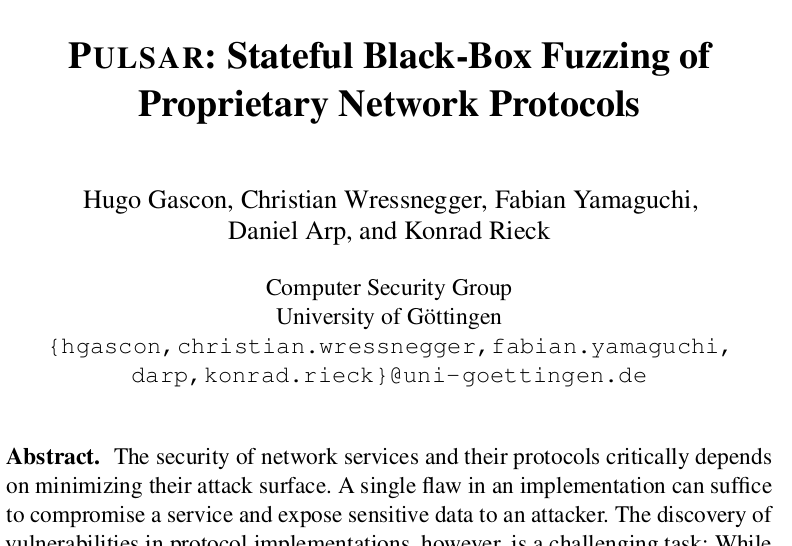
\includegraphics[width=\textwidth]{res/pulsar}
        \caption[Pioniere des Fuzzing mit Machine Learning]{
            Veröffentlichung des ersten Fuzzers mit statistischen Modellen~\cite{thuraisingham_pulsar_2015}
        }
        \label{fig:ml_fuzzing}
    \end{figure}
\end{frame}
\begin{frame}{Pulsar}
    \begin{itemize}
        \item Erster Fuzzer mit \enquote{Machine Learning}
        \item Verwendung von Markov-Modellen
        \item Erkennt und simuliert Zustände
        \item Erkennt und simuliert Nachrichten
        \item Kann sowohl ein Protokoll simulieren, als auch das tatsächliche Protokoll fuzzen
    \end{itemize}
\end{frame}
\section{Demo}\label{sec:demo}
\begin{frame}{Anwendungsfälle für Machine Learning und Fuzzing}
    \begin{itemize}
        \item Generierung von besseren Eingaben mittels Reinforcement Learning
        \item Generierung von Eingaben mit Generative Adversarial Networks
        \item Erlernen von Verhaltensweisen von Programmen mittels Unsupervised Learning
        \item Adaptives Fuzzing mittels Anormalitätserkennung der Ausgaben des zu testenden Programms
        \item Umgehen von Sicherheitsmechanismen durch Erlernen von Vermeidungsstrategien gegen Intrusion Detection Systeme
    \end{itemize}
\end{frame}
\begin{frame}{Limitationen und Herausforderungen von ML und Fuzzing}
    \begin{itemize}
        \item Hohe Rechenanforderungen
        \item Trainingsdatenknappheit in neuen und Nischen Domänen
        \item Model Generalisierung zur Anwendbarkeit auf neue Domänen kann zu ungewolltem overfitting führen
    \end{itemize}
\end{frame}
\begin{frame}{Ausblick}
    \alert{Fuzzing von Netzwerkprotokollen mit Machine Learning}
    \begin{itemize}
        \item Fuzzer kann durch frei verfügbaren Netzwerkverkehr trainiert werden
        \item Eingaben sollen von bereits existierenden Netzwerkprotokollen abgeleitet werden und darin bereits
        enthaltene Fehler reproduzieren
        \item Dynamische Analyse zur Laufzeit des Protokolls soll die Generierung der Eingaben durch reinforcement learning verbessern
        \item Crashes und Bugs sollen gelabelt werden, um die Qualität der Eingaben zu verbessern
        und die Schwere der Bugs zu klassifizieren
    \end{itemize}
\end{frame}
\section{Fragen}\label{sec:fragen}